\documentclass[a4paper,oneside,12pt]{report}
% Package yang diperlukan
\usepackage{fontspec}       % Font sistem untuk XeLaTeX/LuaLaTeX
\usepackage{setspace}       % Pengaturan jarak antarbaris
\usepackage{graphicx}      % Untuk memasukkan gambar
\usepackage{titling}       % Untuk kustomisasi halaman judul
\usepackage{geometry}      % Untuk mengatur margin halaman
\usepackage{listings}      % Untuk menampilkan blok kode
\usepackage{xcolor}        % Untuk menggunakan warna
\usepackage{float}         % Untuk kontrol penempatan float (seperti gambar)
\usepackage{hyperref}      % Untuk membuat hyperlink (URL, referensi)
\usepackage{indentfirst}   % Untuk memberi indentasi pada paragraf pertama setiap seksi
\usepackage{url}           % Untuk format URL
\usepackage{xurl}          % Untuk pemotongan URL panjang agar rapi
\usepackage{fancyhdr}      % Untuk kustomisasi header dan footer
\usepackage{tocloft}       % Untuk kustomisasi Daftar Isi
\usepackage{bookmark}      % Untuk manajemen bookmark PDF yang lebih baik

% Font dan spasi standar laporan praktikum
\setmainfont{TeX Gyre Termes}
\onehalfspacing

%======================================================================
% PENGATURAN GEOMETRI HALAMAN
%======================================================================
\geometry{left=3cm, right=2.5cm, top=2cm, bottom=2.5cm}
\sloppy

%======================================================================
% PENGATURAN WARNA UNTUK BLOK KODE
%======================================================================
\definecolor{codegreen}{rgb}{0,0.6,0}
\definecolor{codegray}{rgb}{0.5,0.5,0.5}
\definecolor{codepurple}{rgb}{0.58,0,0.82}
\definecolor{backcolour}{rgb}{0.95,0.95,0.92}
\definecolor{darkblue}{rgb}{0,0,0.6}

%======================================================================
% PENGATURAN BLOK KODE (LISTINGS)
%======================================================================
\lstdefinestyle{commonstyle}{
    backgroundcolor=\color{backcolour},
    breakatwhitespace=false,
    breaklines=true,
    captionpos=b,
    keepspaces=true,
    numbers=left,
    numbersep=5pt,
    showspaces=false,
    showstringspaces=false,
    showtabs=false,
    tabsize=2,
    frame=single,
    basicstyle=\ttfamily\footnotesize,
    numberstyle=\tiny\color{codegray},
    columns=flexible,
    postbreak=\mbox{\textcolor{red}{$\hookrightarrow$}\space},
    breakindent=0pt,
    breakautoindent=false
}

%======================================================================
% PENGATURAN LAIN-LAIN
%======================================================================
\newcommand{\customfbox}[1]{%
  \setlength{\fboxsep}{0pt}%
  \setlength{\fboxrule}{0.5pt}%
  \fcolorbox{black}{white}{#1}%
}
\renewcommand{\figurename}{Gambar}
\renewcommand{\thefigure}{\arabic{figure}}
\hypersetup{
    colorlinks=true,
    linkcolor=black,
    filecolor=black,
    urlcolor=black,
    citecolor=black,
    pdftitle={Laporan Praktikum PPG Pertemuan 3},
    pdfpagemode=UseOutlines,
    breaklinks=true
}
\pagestyle{fancy}
\fancyhf{}
\fancyfoot[C]{\thepage}
\renewcommand{\headrulewidth}{0pt}
\fancypagestyle{plain}{
    \fancyhf{}
    \fancyfoot[C]{\thepage}
    \renewcommand{\headrulewidth}{0pt}
}
\renewcommand{\contentsname}{Daftar Isi}
\renewcommand{\bibname}{Daftar Pustaka}
\renewcommand{\thechapter}{}
\renewcommand{\chaptername}{}
\renewcommand{\thesection}{\arabic{chapter}.\arabic{section}}
\renewcommand{\thesubsection}{\thesection.\arabic{subsection}}
\setcounter{secnumdepth}{3}
\setcounter{tocdepth}{3}
\renewcommand{\cftchapdotsep}{\cftdotsep}
\renewcommand{\cftchapleader}{\cftdotfill{\cftchapdotsep}}
\setlength{\cftchapindent}{0em}
\setlength{\cftsecindent}{2em}
\setlength{\cftsubsecindent}{4em}
\setlength{\cftchapnumwidth}{0em}
\setlength{\cftsecnumwidth}{2.5em}
\setlength{\cftsubsecnumwidth}{3.2em}
\renewcommand{\cftchappresnum}{}
\renewcommand{\cftchapaftersnum}{}
\newcommand{\tocboldsection}[1]{%
  \protect\renewcommand{\protect\cftchapfont}{\protect\bfseries}%
  #1%
  \protect\renewcommand{\protect\cftchapfont}{}%
}
\pdfstringdefDisableCommands{\def\tocboldsection#1{#1}}

%======================================================================
% AWAL DOKUMEN
%======================================================================
\begin{document}

% Halaman Judul
\newgeometry{left=3cm, right=2.5cm, top=2.5cm, bottom=3cm}
\begin{titlingpage}
\begin{spacing}{1}
\begin{center}
\vspace*{0.2cm}
{\large \textbf{\MakeUppercase{Laporan Praktikum}}} \\[0.4cm]
{\large \textbf{\MakeUppercase{PRAKTIKUM PENGEMBANGAN GAME}}} \\[0.4cm]
{\large \textbf{\MakeUppercase{Pertemuan 3}}} \\[0.4cm]
{\large \textbf{\MakeUppercase{VARIABLE \& CONDITION}}} \\[1.5cm]


\includegraphics[height=7cm]{images/UGM.png} \\[0.7cm]

{\normalsize \textbf{Disusun oleh:}} \\[0.4cm]
\begin{tabular}{@{}l l @{}}
  \textbf{Nama}           & : Hafidz Rizqullah Prasetya \\
  \textbf{NIM}            & : 24/535493/SV/24243 \\
  \textbf{NIU}            & : 535493 \\
  \textbf{Kelas}          & : PL5A1 \\
  \textbf{Dosen Pengampu} & : Yusron Fuadi, S.Sn., M.Sn. \\
  \textbf{Asisten}        & : Ezra Bariq Rizqullah / Ikhwan Hanif Firdaus \\
\end{tabular} \\[1.2cm]

{\normalsize \textbf{PROGRAM STUDI D-IV}} \\[0.2cm]
{\normalsize \textbf{TEKNOLOGI REKAYASA PERANGKAT LUNAK}} \\[0.2cm]
{\normalsize \textbf{DEPARTEMEN TEKNIK ELEKTRO DAN INFORMATIKA}} \\[0.2cm]
{\normalsize \textbf{SEKOLAH VOKASI}} \\[0.2cm]
{\normalsize \textbf{UNIVERSITAS GADJAH MADA}} \\[0.2cm]
{\normalsize \textbf{YOGYAKARTA}} \\[0.2cm]
{\normalsize \textbf{2026}} \\[1.2cm]
\end{center}
\end{spacing}
\end{titlingpage}
\restoregeometry

\thispagestyle{empty}
\clearpage
\stepcounter{page}
\thispagestyle{empty}

% --- Daftar Isi ---
\addcontentsline{toc}{chapter}{Daftar Isi}
\tableofcontents
\clearpage

% Mengatur penomoran halaman menjadi arab dan mulai dari 3
\pagenumbering{arabic}
\setcounter{page}{3}

\chapter[Tujuan Praktikum]{Tujuan Praktikum}
\begin{enumerate}
   \item Mahasiswa mampu membuat dan mengonfigurasi project baru berbasis template Third Person dengan format penamaan standar \textbf{NAMA\_NIU\_PPG} di Unreal Engine 5.8 \cite{modul3}.
   \item Mahasiswa mampu menyiapkan level dasar yang meliputi pembuatan struktur folder Maps, Level baru, pencahayaan Env.\ Light Mixer, Landscape, dan penempatan Player Start \cite{modul3,epic-levels}.
   \item Mahasiswa mampu membuat Blueprint Actor (\texttt{BP\_Box}), memahami siklus eksekusi Event BeginPlay dan Event Tick, serta mengelola variabel tipe data primitif maupun mengenal konsep Struct Variable \cite{modul3,epic-variables}.
   \item Mahasiswa mampu menerapkan kontrol alur logika kondisional menggunakan node Branch, menangani input Keyboard, serta mengimplementasikan perubahan transformasi (Scale) objek secara real-time \cite{modul3,epic-flow}.
\end{enumerate}
\clearpage

\chapter{Dasar Teori}

\section{Project Third Person dan Setup Level Baru}
Praktikum kali ini saya kerjakan dari template \textbf{Third Person} pada kategori Games di Unreal Project Browser. Template IntroToUnreal peninggalan pertemuan 2 saya tinggalkan karena bug pada 3D model karakternya menghambat materi Rigging/Retargeting berikutnya \cite{modul3}. Project Name diisi dengan format \textbf{NAMA\_NIU\_PPG}, sehingga project saya bernama \texttt{HAFIDZ\_535493\_PPG}.

Bedanya dengan pertemuan 2 yang langsung membuka tutorial interaktif, project Third Person berangkat dari level contoh yang relatif kosong, jadi level disiapkan manual: folder \textbf{Maps} dibuat di Content Drawer, lalu file \textbf{Level} baru dibuat di dalamnya lewat klik kanan \cite{modul3}. Level di Unreal sendiri adalah wadah berisi semua actor (mesh, light, camera, Player Start) yang tampil di scene, dan setiap Level tersimpan sebagai file \texttt{.umap} \cite{epic-levels}.

Untuk pencahayaan dasar, Level baru saya buka, menu \textbf{Windows} di kiri atas editor saya klik, lalu \textbf{Env.\ Light Mixer} saya buka. Semua tombol \textbf{Create} di window tersebut (Sky Light, Directional Light, Sky Atmosphere, Volumetric Cloud, Exponential Height Fog) ditekan supaya level langsung punya pencahayaan lingkungan yang otomatis dan realistis \cite{modul3}.

Untuk area pijakan dan titik kemunculan pemain, mode \textbf{Landscape} dipakai untuk membuat dataran berukuran \textbf{7x7 Quads, 8x8 Component, Section 1x1}. GameMode diatur ke \textbf{BP\_FirstPersonGameMode}, lalu aktor \textbf{Player Start} ditempatkan di atas tanah \cite{modul3}. Objek kecil berbentuk bendera ini menandai posisi awal spawn karakter saat permainan dijalankan, dengan ikon yang terletak di sebelah kiri tombol Play pada toolbar \cite{epic-place}.

\section{Blueprint, Event BeginPlay, dan Event Tick}
Sebelum menulis logika, folder \textbf{Blueprints} disiapkan dulu sebagai tempat semua file kode. File Blueprint memakai prefix \textbf{BP\_} sesuai konvensi penamaan resmi Epic Games \cite{epic-naming}, dan Blueprint yang dibuat bernama \texttt{BP\_Box}. Bentuk awal Blueprint masih kosong, hanya berupa titik pivot, jadi tombol \textbf{+ Add} di panel Components ditekan untuk menambahkan komponen \textbf{Cube} supaya wujudnya kelihatan sebagai kotak saat di-spawn ke map \cite{modul3}.

Kode di Unreal Engine 5 butuh event sebagai pemicu supaya bisa jalan. Dua event bawaan yang selalu ada di tab \textbf{Event Graph} adalah \textbf{Event BeginPlay} yang dieksekusi satu kali saat game atau objek dimulai, dan \textbf{Event Tick} yang dieksekusi terus-menerus setiap frame \cite{modul3}. Pembuktiannya sederhana: Blueprint di-drag and drop ke dalam level, node \textbf{Print String} dipasang, dan kalau teks debug muncul di layar saat Play, berarti kode di Event Graph berhasil dieksekusi \cite{modul3,epic-unreal}.

Actor adalah objek dasar yang bisa ditempatkan di level, sedangkan Pawn/Character adalah actor yang bisa dikendalikan input pemain \cite{epic-actors}. Bedanya kepakai waktu saya membaca hubungan antara \texttt{BP\_Box} yang dibuat dan karakter Third Person yang dipakai menguji input keyboard.

\section{Variabel di Blueprint}
Variabel di Blueprint menyimpan data yang dipakai logika. Pilihannya banyak, dari tipe primitif seperti Boolean, Integer, Float, String, dan Vector, sampai tipe tambahan seperti \textbf{Transform} yang otomatis membungkus tiga variabel sekaligus (Location, Rotation, Scale), \textbf{Enum}, dan \textbf{user defined class} \cite{modul3,epic-variables}. Variabel baru saya buat dari panel \textbf{My Blueprint} dengan mengklik ikon \textbf{(+)}, lalu tipe datanya dipilih dari daftar drop-down. Modul meminta variabel bertipe \textbf{Boolean} ditambahkan pada \texttt{BP\_Box} sebagai bahan percobaan Branch \cite{modul3}.

Selain variabel tunggal, modul juga memperkenalkan \textbf{Struct Variable}: child Blueprint yang menampung beberapa variabel beda jenis dalam satu wadah, mirip List atau Dictionary kompleks di Python \cite{modul3}. Materinya masih pengenalan dan baru dibahas lebih dalam pada pertemuan berikutnya, jadi cukup dipahami idenya: satu Struct bisa menyimpan String, Integer, dan Boolean sekaligus dalam satu paket.

\section{Branch dan Kontrol Alur}
Node baru ditambahkan dengan \textbf{klik kanan} pada area kosong Event Graph, lalu mengetik kata kunci seperti ``if'', ``get \textless nama\_variabel\textgreater'', ``set \textless nama\_variabel\textgreater'', atau ``print string'' \cite{modul3}. Navigasi kanvas memakai klik kanan yang ditahan sambil menggerakkan mouse (panning) supaya graph yang panjang tetap gampang dijelajahi.

Node \textbf{Branch} adalah padanan \textit{if} pada pseudo-code: satu pin eksekusi masuk, satu pin kondisi bertipe Boolean, dan dua pin eksekusi keluar yaitu \textbf{True} dan \textbf{False} \cite{modul3,epic-flow}. Alur hanya lewat ke salah satu cabang sesuai nilai kondisinya.

Contoh paling sederhana di modul memakai \textbf{Event Tick} yang disambung ke logika penekanan tombol. Kata ``keyboard'' saya ketik pada menu tambah node untuk memunculkan \textbf{Keyboard R} dari kategori Input Events \cite{epic-input}. Pin Pressed/Released dari node tersebut dipakai mengubah variabel Boolean lewat node \textbf{Set}, lalu variabel itu dibaca lewat node \textbf{Get} dan dimasukkan ke pin kondisi Branch (dapat ditambahkan node \textbf{Not Boolean} bila logika ingin dibalik). Dari pin True/False dua kabel eksekusi disambungkan ke dua node \textbf{Print String} berbeda, sehingga teks yang tercetak di layar berganti tergantung tombol R sedang ditekan atau tidak \cite{modul3}.

Di luar Branch masih ada node flow control lain: \textbf{Switch} (satu input, banyak output Case untuk mencocokkan nilai), \textbf{Do Once} (eksekusi sekali sampai di-reset), \textbf{Flip Flop} (output A dan B aktif bergantian), dan \textbf{Gate} (pintu Open/Close/Toggle yang mengatur apakah alur boleh lewat) \cite{modul3,epic-flow}. Keempatnya ditandai opsional dan boleh dipelajari mandiri kalau waktu praktikum tidak cukup.

\section{Penerapan If/Else Real-Time dan Konvensi Penamaan}
Tugasnya mengaplikasikan if/else untuk mengubah scale, rotasi, atau lokasi mesh secara real-time lewat kode pada Event Tick \texttt{BP\_Box}. Variabel float bernama \textbf{ScaleTarget} (atau \textit{scale target}) dengan default value \textbf{0.1} ditambahkan, lalu Event Tick dipakai menggeser nilai Scale mesh menuju target tersebut lewat node matematika seperti pengurangan atau Lerp \cite{modul3}. Satu trik penting dari modul: klik kanan pada pin konektor operasi bilangan untuk mengonversi tipe data (misalnya Vector ke Float) supaya operasi matematikanya tidak error merah dan bisa jalan \cite{modul3}.

Modul memberi catatan jujur bahwa cara ini bukan best practice dan hanya untuk keperluan praktikum: mengubah transformasi di dalam Event Tick tanpa Delta Time atau Timeline membuat pergerakan tidak konsisten di beda frame rate dan membebani performa \cite{modul3}. Game dari editor sendiri dijalankan lewat tombol Play atau project standalone untuk pengujian yang lebih bersih \cite{epic-running}.

Supaya project tetap rapi, konvensi penamaan resmi Epic saya ikuti: prefix \texttt{BP\_} untuk Blueprint, \texttt{M\_} untuk Material, \texttt{T\_} untuk Texture, dan seterusnya \cite{epic-naming}. Kebiasaan kecil ini membuat aset gampang dicari saat project membesar.

\clearpage

\chapter[\tocboldsection{Hasil dan Pembahasan}]{Hasil dan Pembahasan}

Bab ini berisi dokumentasi praktikum Variable \& Condition sesuai Modul Pertemuan 3. Seluruh langkah dikerjakan di Unreal Engine 5.8 pada project \texttt{HAFIDZ\_535493\_PPG} dari template Third Person, dan tiap langkah didokumentasikan dengan screenshot berikut keterangan singkatnya.

\section{Dokumentasi Praktikum}

\subsection{Basic Setup: Project, Maps, Level, dan Lighting}

\begin{enumerate}
    \item \textbf{Membuat project Third Person bernama HAFIDZ\_535493\_PPG.} Unreal Project Browser dibuka, kategori \textbf{Games} dan template \textbf{Third Person} dipilih, lalu Project Name diisi dengan format NAMA\_NIU\_PPG. Template ini saya pilih karena IntroToUnreal punya bug pada 3D model karakter yang menghambat materi Rigging/Retargeting.

\begin{figure}[H]
    \centering
    \customfbox{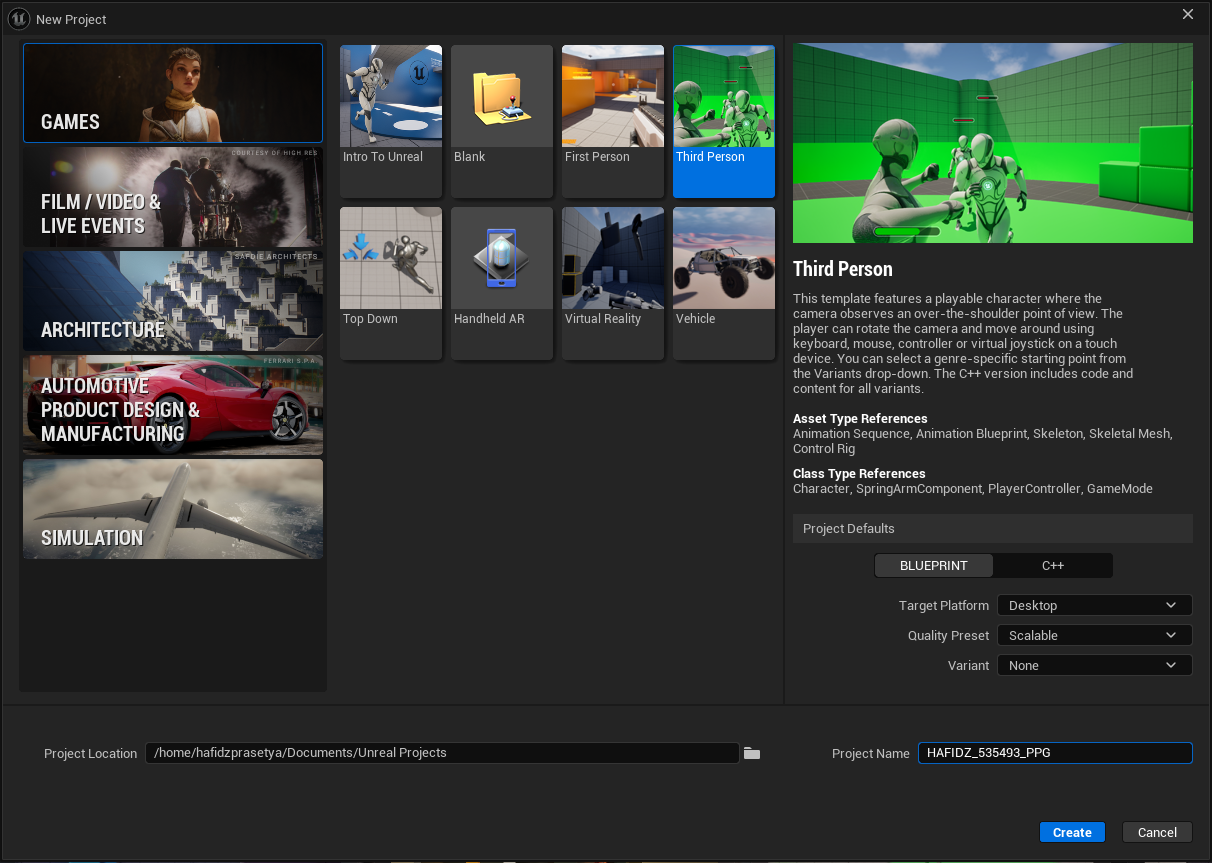
\includegraphics[width=0.9\textwidth]{images/ss-01-project-thirdperson.png}}
    \caption{Jendela New Project: kategori Games, template Third Person, dan Project Name HAFIDZ\_535493\_PPG.}
    \label{fig:ss-project}
\end{figure}

    \item \textbf{Membuat folder Maps dan Level baru.} Di Content Drawer area kosong diklik kanan untuk membuat folder \textbf{Maps}, lalu di dalam folder tersebut file \textbf{Level} baru bernama \textbf{L\_Main} dibuat lewat klik kanan sebagai arena kerja praktikum ini.

\begin{figure}[H]
    \centering
    \customfbox{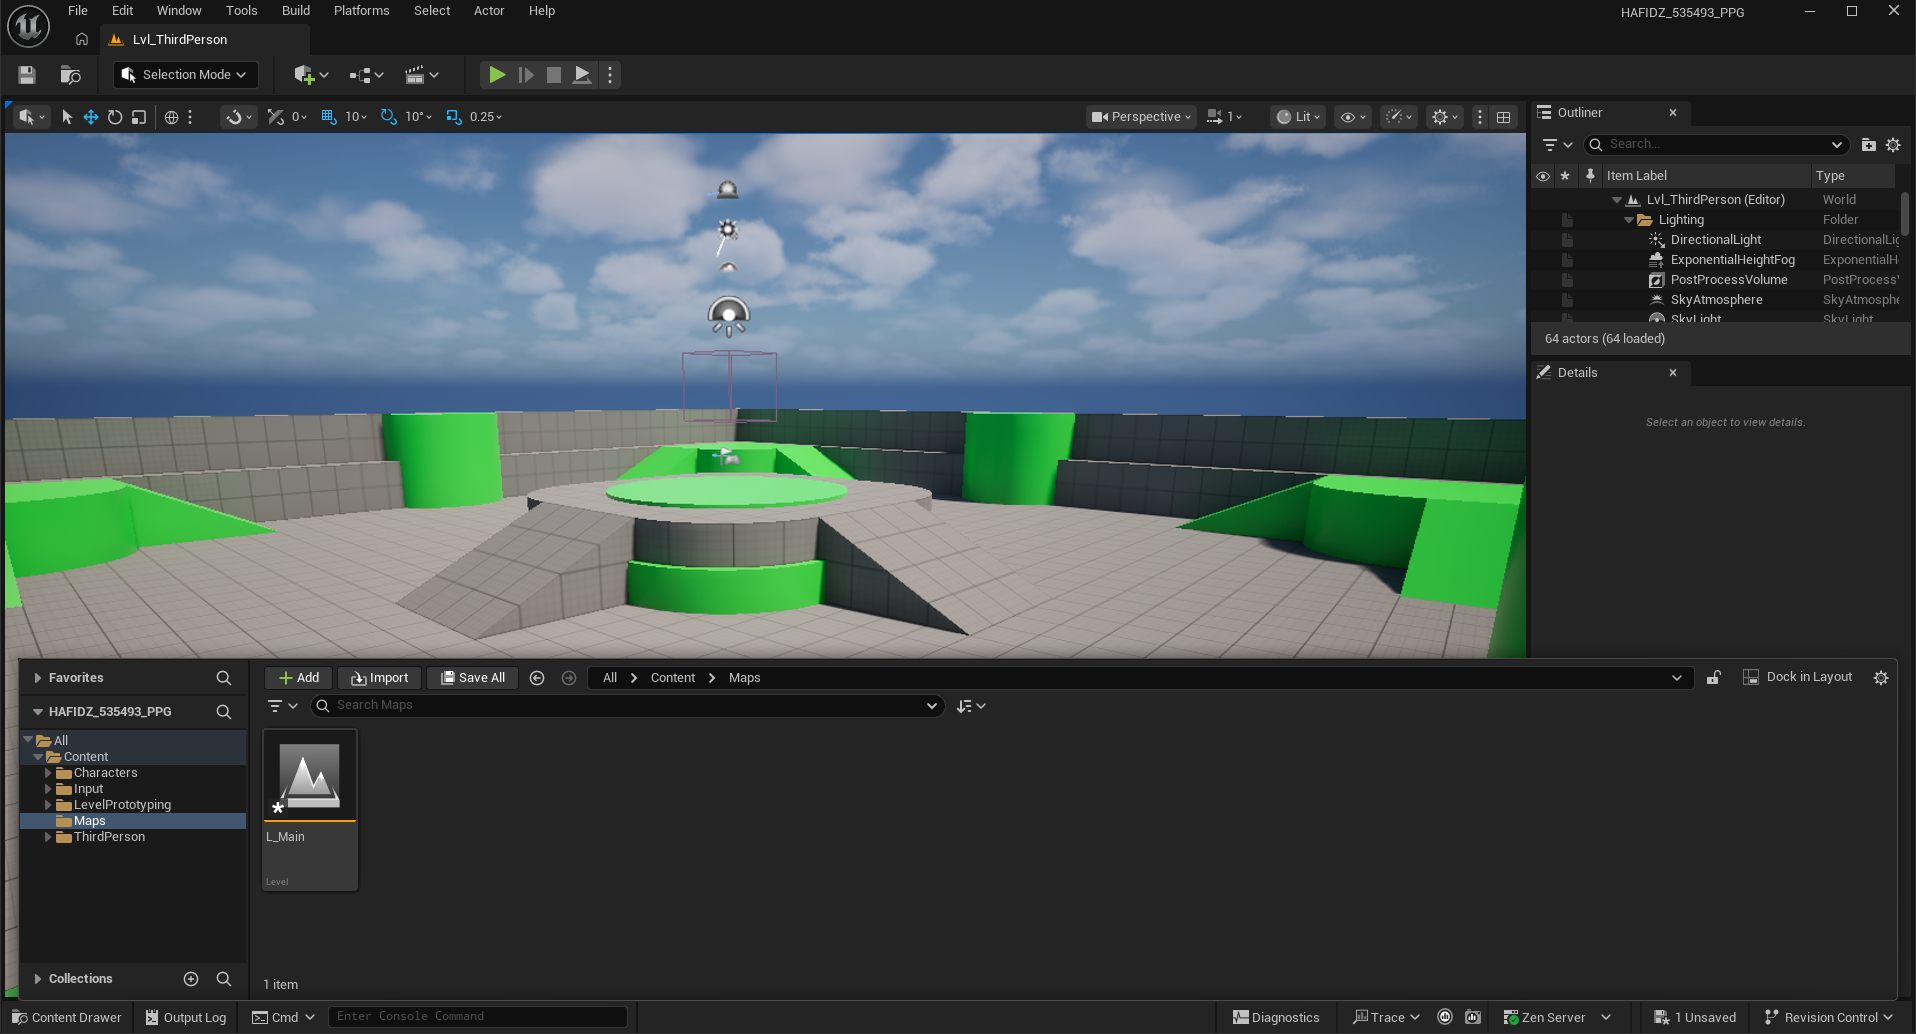
\includegraphics[width=0.9\textwidth]{images/ss-02-maps-level.png}}
    \caption{Folder Maps di Content Drawer beserta file Level baru L\_Main di dalamnya.}
    \label{fig:ss-maps}
\end{figure}

    \item \textbf{Membuat pencahayaan dasar lewat Env.\ Light Mixer.} Level baru dibuka, menu \textbf{Windows} di kiri atas editor diklik, lalu \textbf{Env.\ Light Mixer} dibuka. Semua tombol \textbf{Create} di window tersebut saya tekan supaya Sky Light, Directional Light, Sky Atmosphere, Volumetric Cloud, dan Exponential Height Fog langsung terpasang.

\begin{figure}[H]
    \centering
    \customfbox{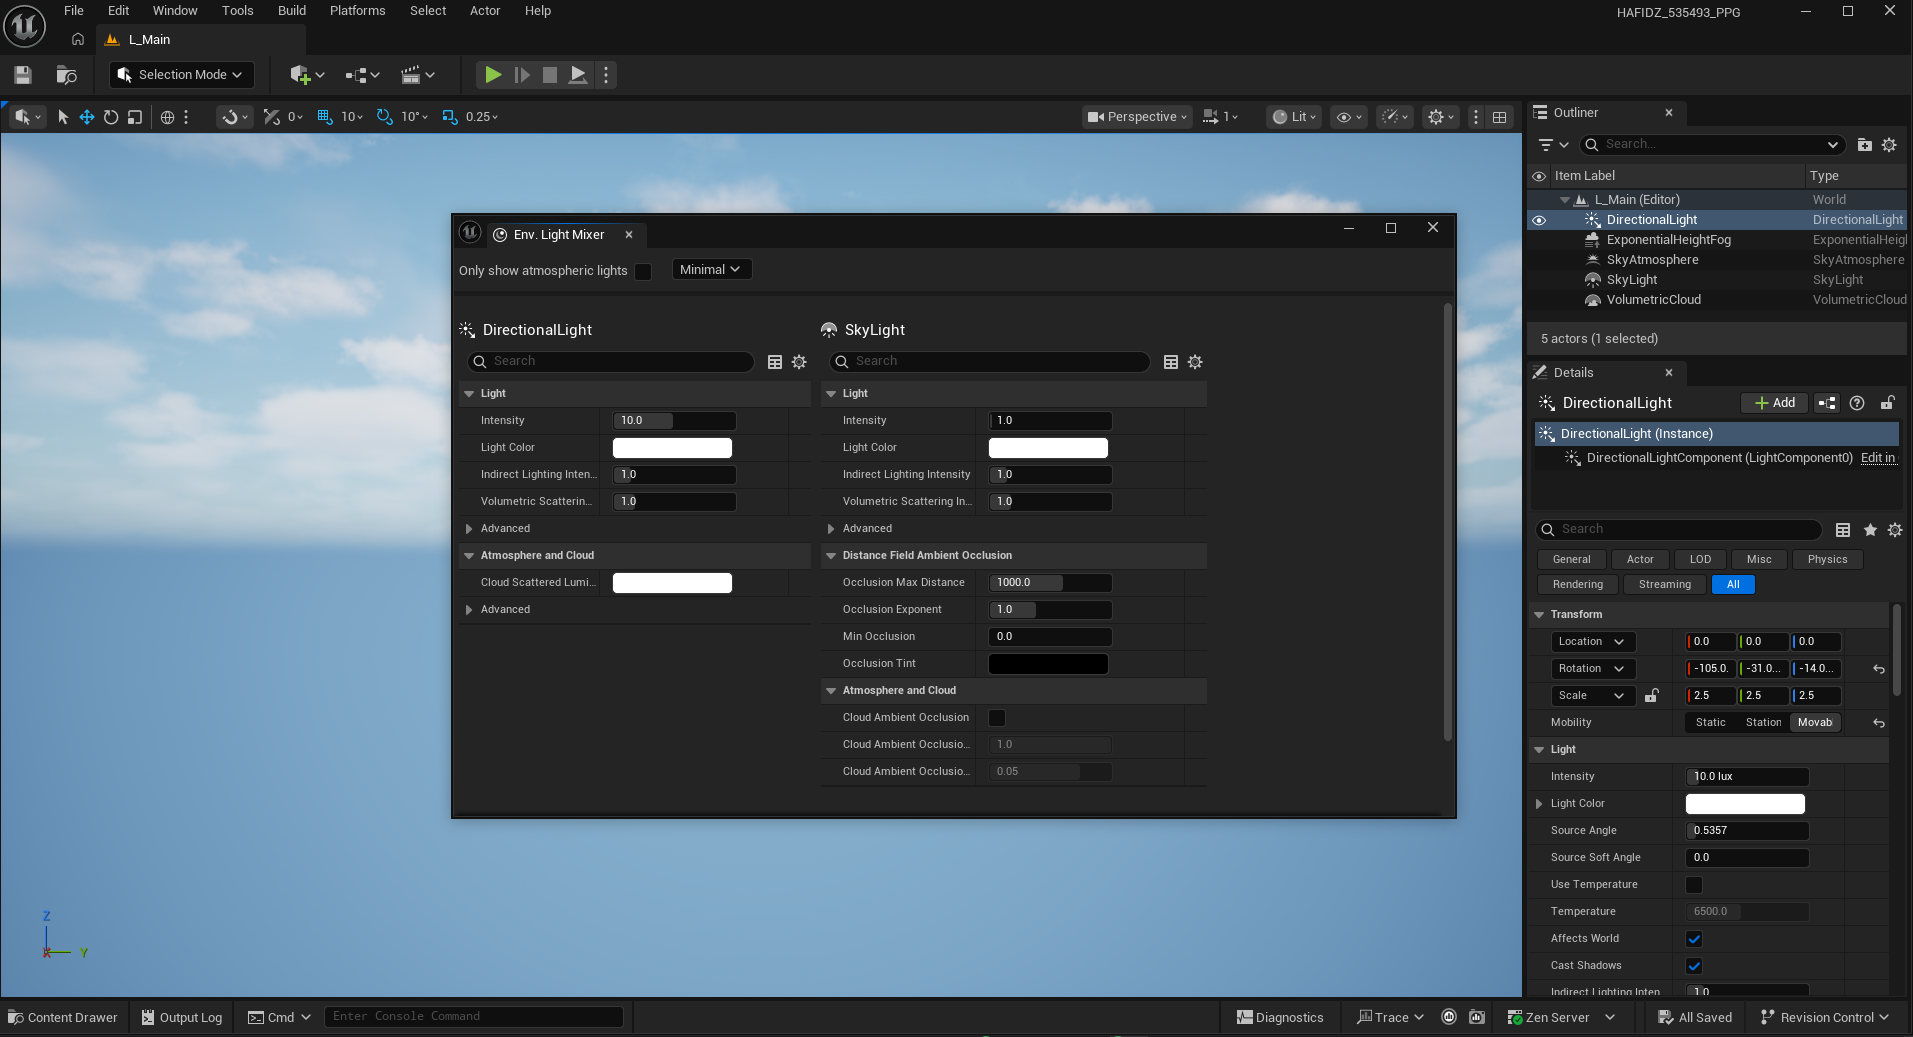
\includegraphics[width=0.9\textwidth]{images/ss-03-env-light-mixer.png}}
    \caption{Panel Env.\ Light Mixer dengan seluruh opsi pencahayaan lingkungan yang sudah di-Create.}
    \label{fig:ss-lightmixer}
\end{figure}

    \item \textbf{Menambahkan Landscape dan Player Start.} Dari \textbf{Landscape Mode} landscape berukuran \textbf{7x7 Quads, 8x8 Component, Section 1x1} dibuat, gamemode diganti ke \textbf{BP\_FirstPersonGameMode}, lalu \textbf{Player Start} ditaruh ke Level sebagai titik spawn karakter. Ikonnya saya ambil dari sebelah kiri tombol Play.

\begin{figure}[H]
    \centering
    \customfbox{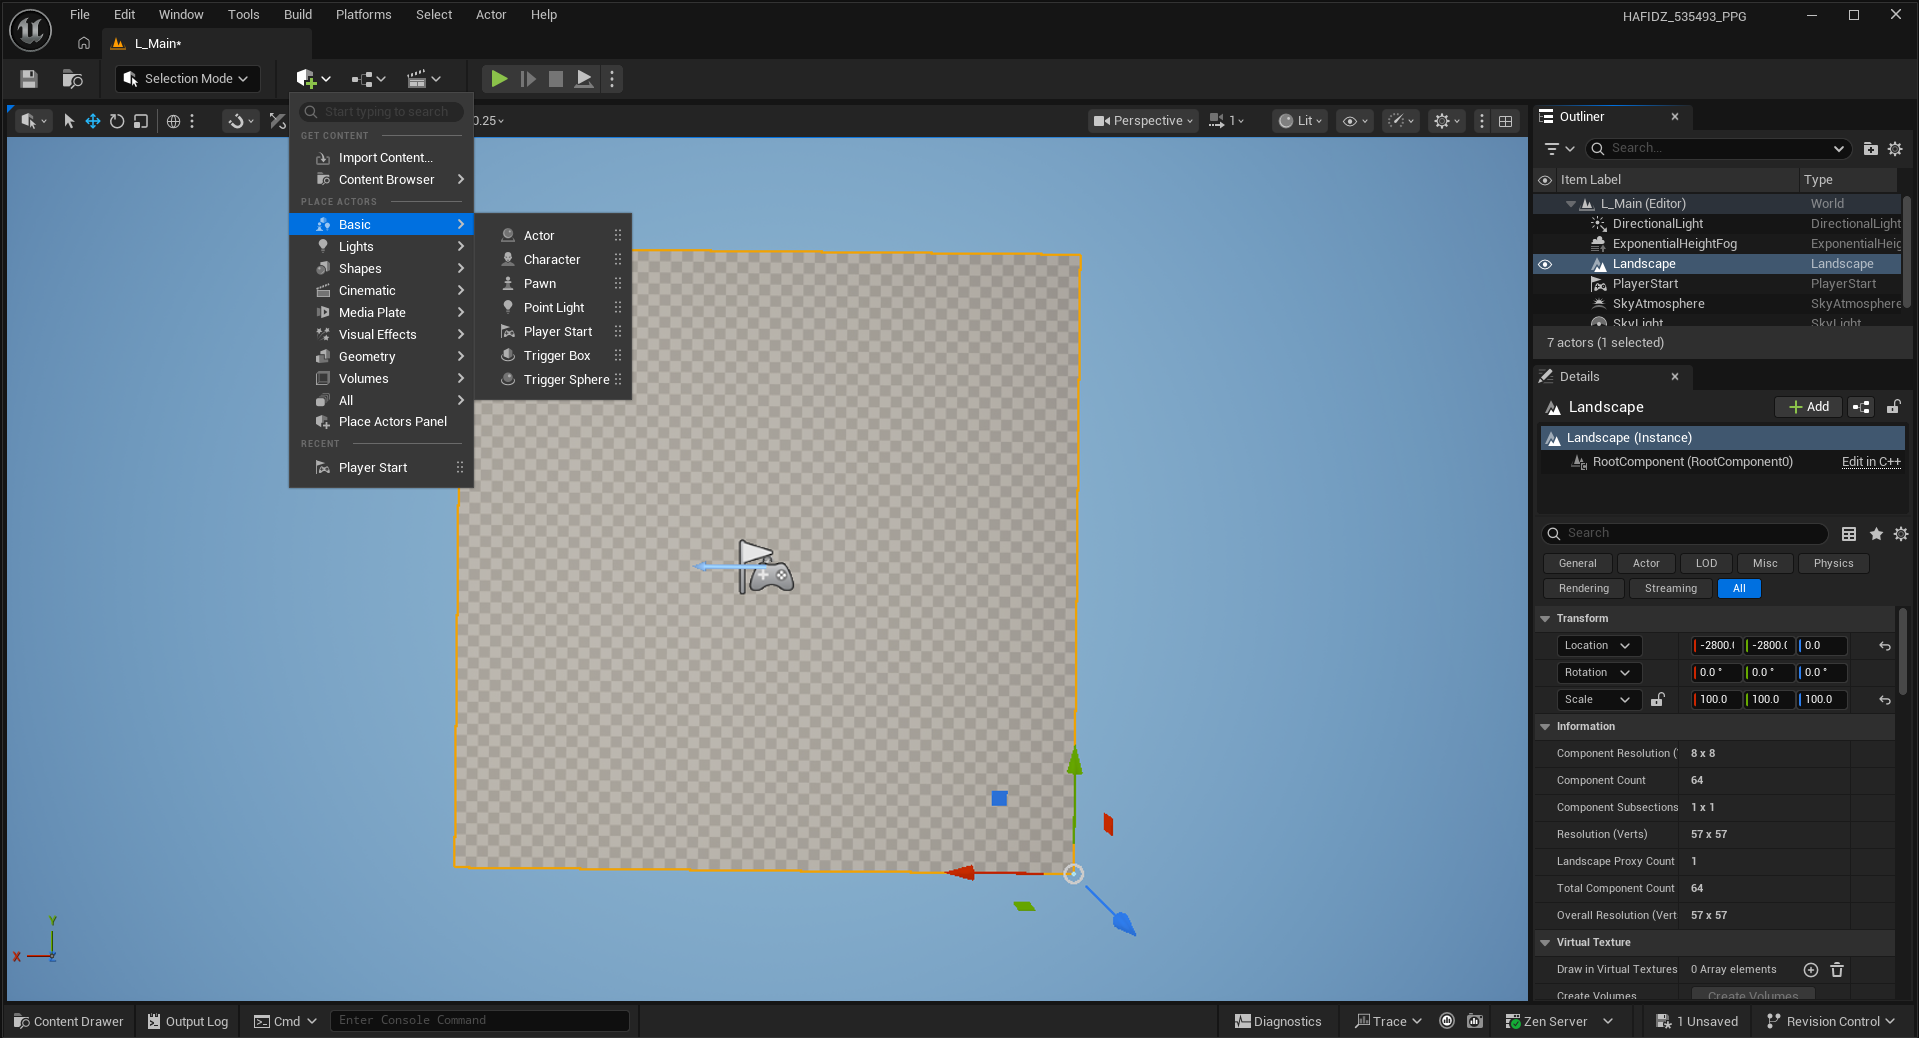
\includegraphics[width=0.9\textwidth]{images/ss-04-landscape-playerstart.png}}
    \caption{Landscape 7x7 di Level beserta actor Player Start sebagai titik spawn pemain.}
    \label{fig:ss-landscape}
\end{figure}
\end{enumerate}

\subsection{Blueprint, Event, dan Variabel}

\begin{enumerate}
    \item \textbf{Membuat BP\_Box berisi komponen Cube.} Folder \textbf{Blueprints} dibuat, Blueprint Class baru bernama \textbf{BP\_Box} ditambahkan, lalu di panel Components tombol \textbf{+ Add} ditekan untuk menambahkan komponen \textbf{Cube} supaya wujudnya kelihatan sebagai kotak saat di-spawn ke map.

\begin{figure}[H]
    \centering
    \customfbox{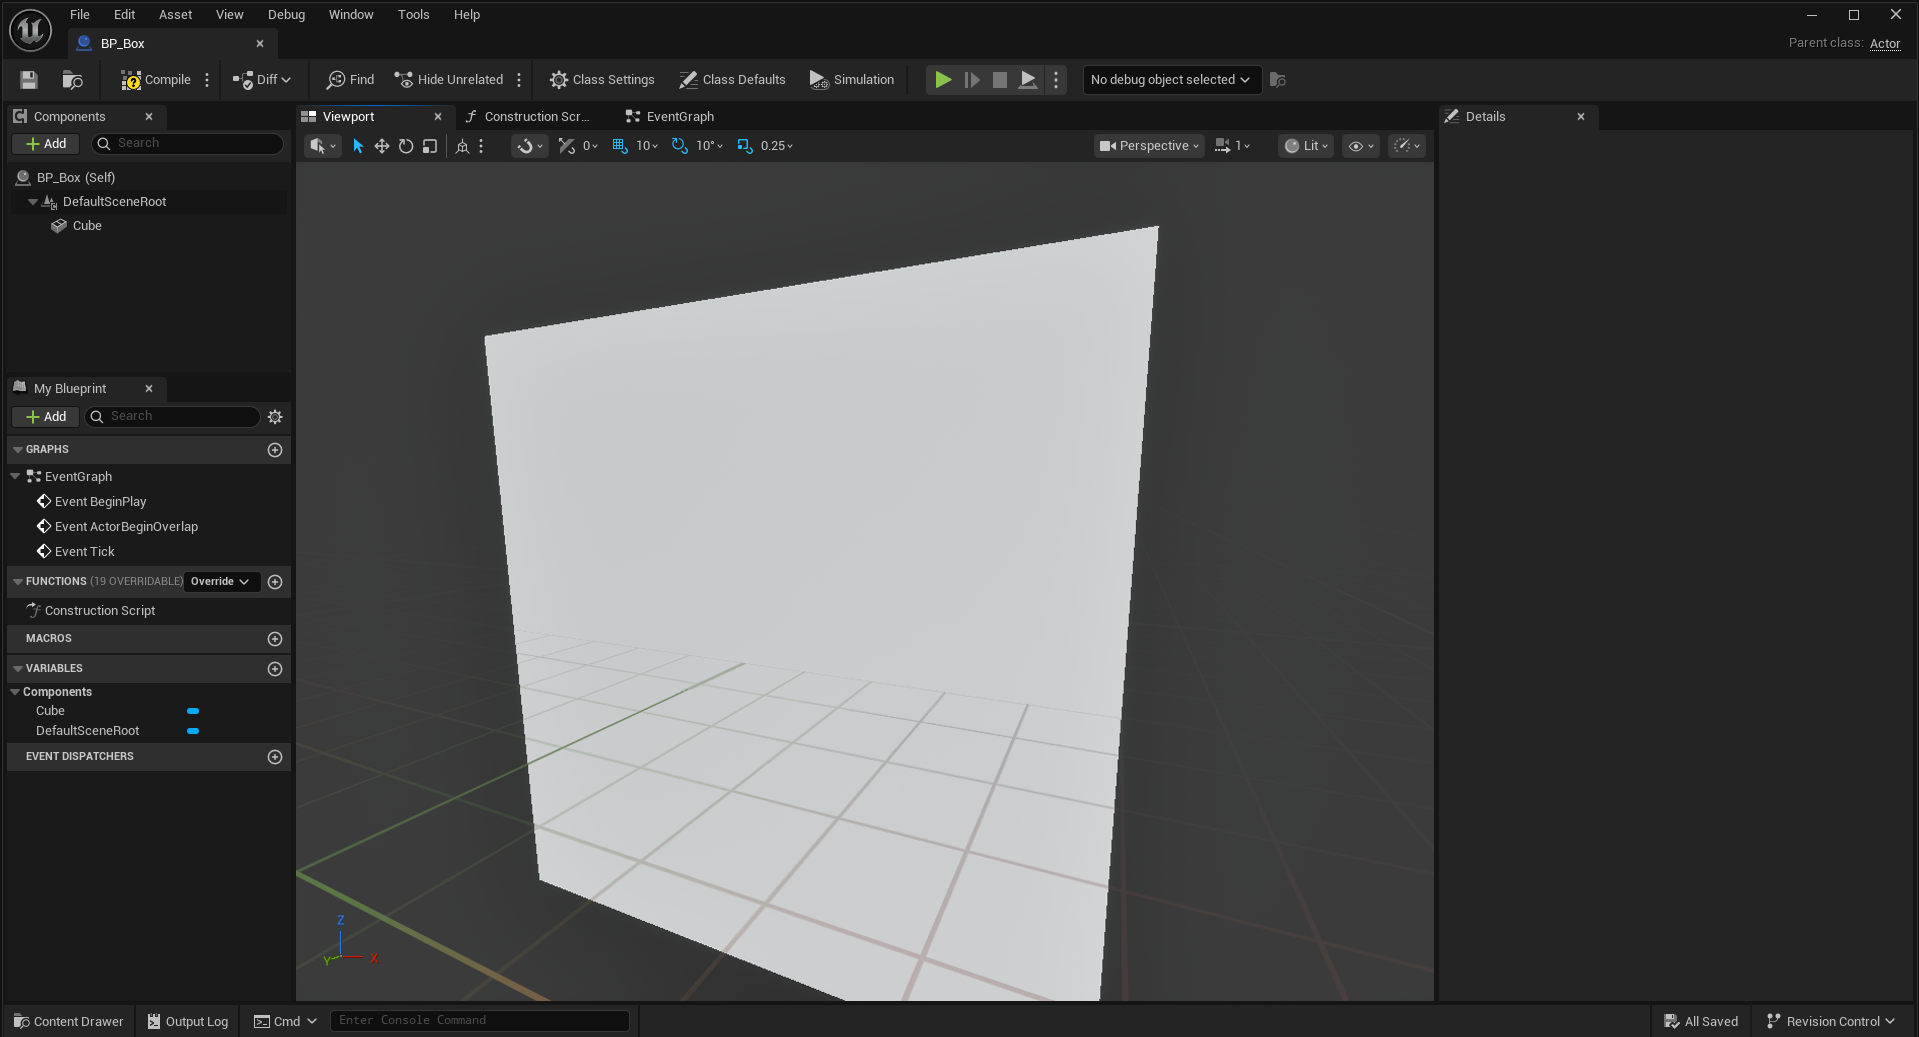
\includegraphics[width=0.9\textwidth]{images/ss-05-bp-box-cube.png}}
    \caption{Editor BP\_Box: folder Blueprints, komponen Cube yang ditambahkan lewat tombol Add.}
    \label{fig:ss-bpbox}
\end{figure}

    \item \textbf{Mencoba Event BeginPlay, Event Tick, dan Print String.} Di tab \textbf{Event Graph} dua node merah bawaan dipakai: \textbf{Event BeginPlay} (jalan sekali) dan \textbf{Event Tick} (jalan tiap frame). \texttt{BP\_Box} saya drag and drop ke dalam level dan node \textbf{Print String} dipasang; teks debug yang muncul di layar membuktikan graph berjalan.

\begin{figure}[H]
    \centering
    \customfbox{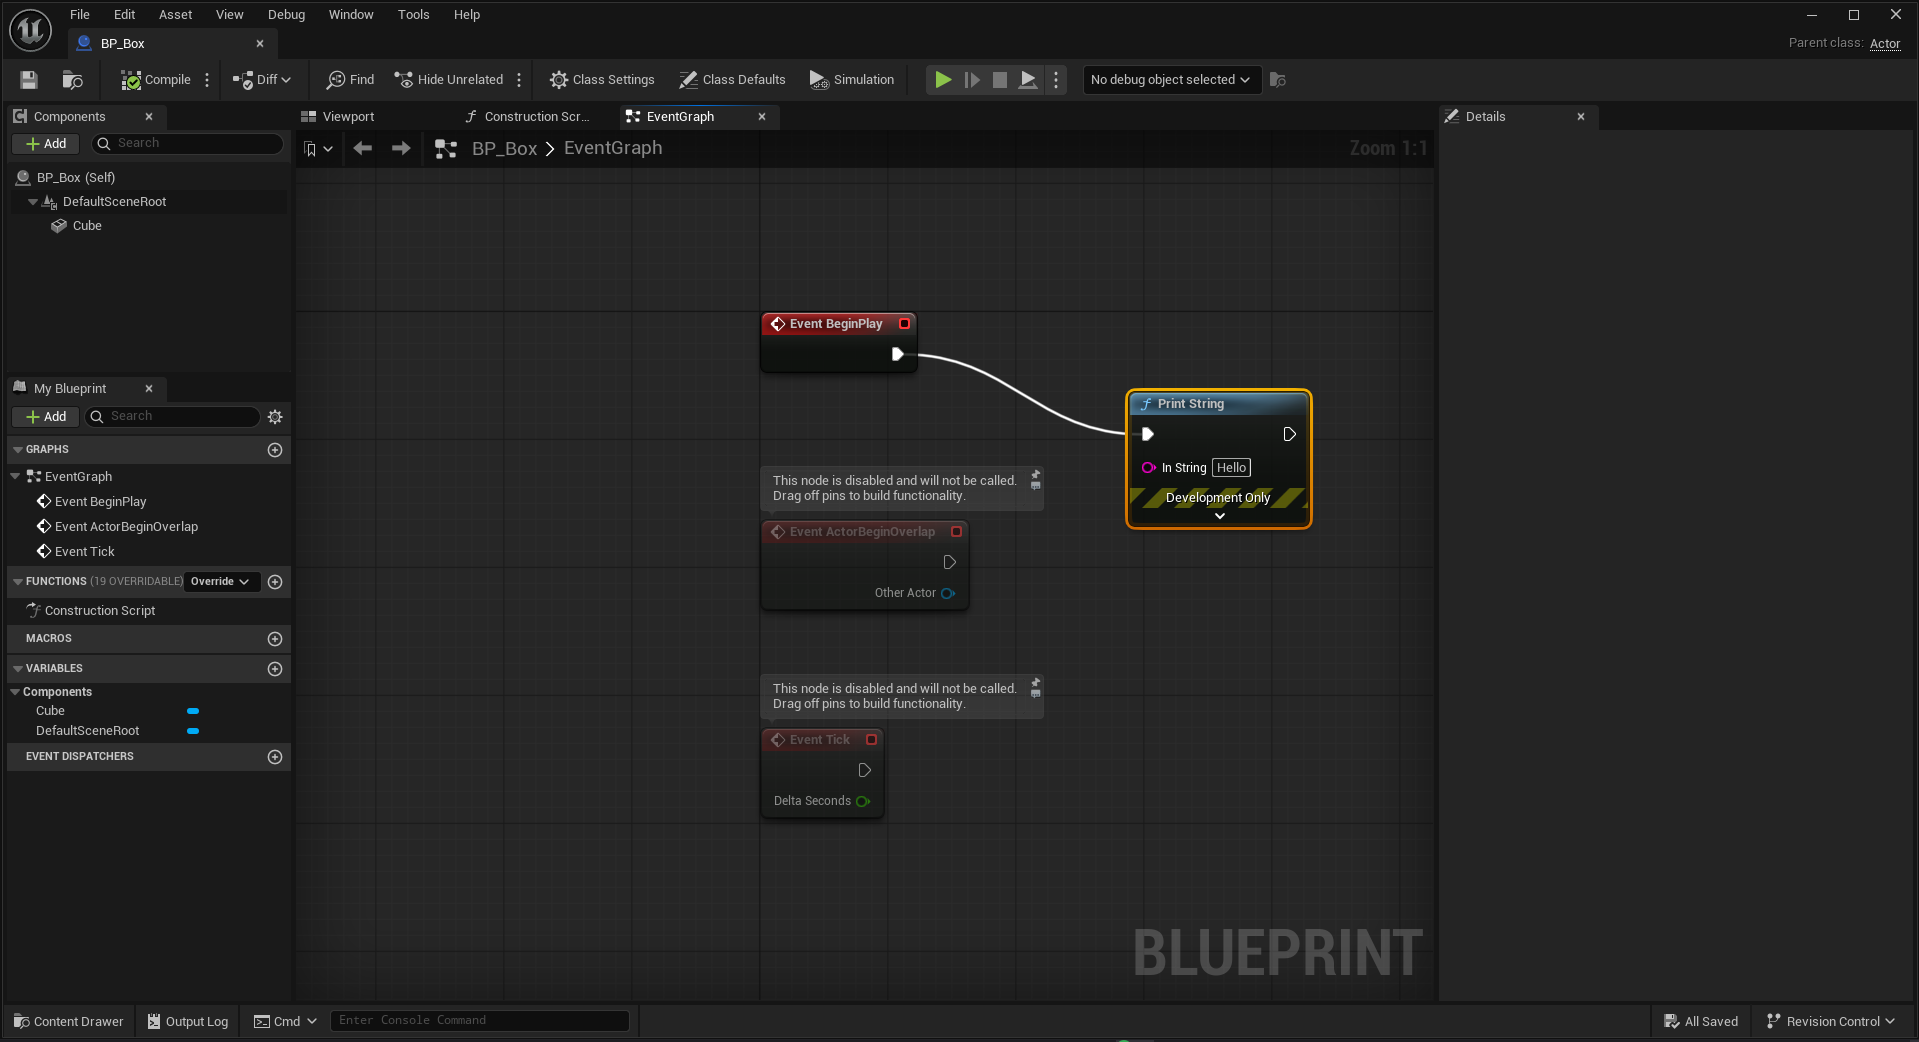
\includegraphics[width=0.9\textwidth]{images/ss-06-event-beginplay-tick.png}}
    \caption{Event Graph BP\_Box: Event BeginPlay dan Event Tick beserta teks debug Print String di viewport.}
    \label{fig:ss-event}
\end{figure}

    \item \textbf{Menambahkan variabel boolean pada BP\_Box.} Dari panel \textbf{My Blueprint} ikon \textbf{(+)} diklik untuk membuat variabel baru bertipe \textbf{Boolean} bernama \textbf{IsActive}. Daftar drop-down tipenya menampilkan pilihan primitif (Boolean, Integer, Float, String, Vector) sampai tipe kompleks seperti Transform, Enum, dan Class Reference.

\begin{figure}[H]
    \centering
    \customfbox{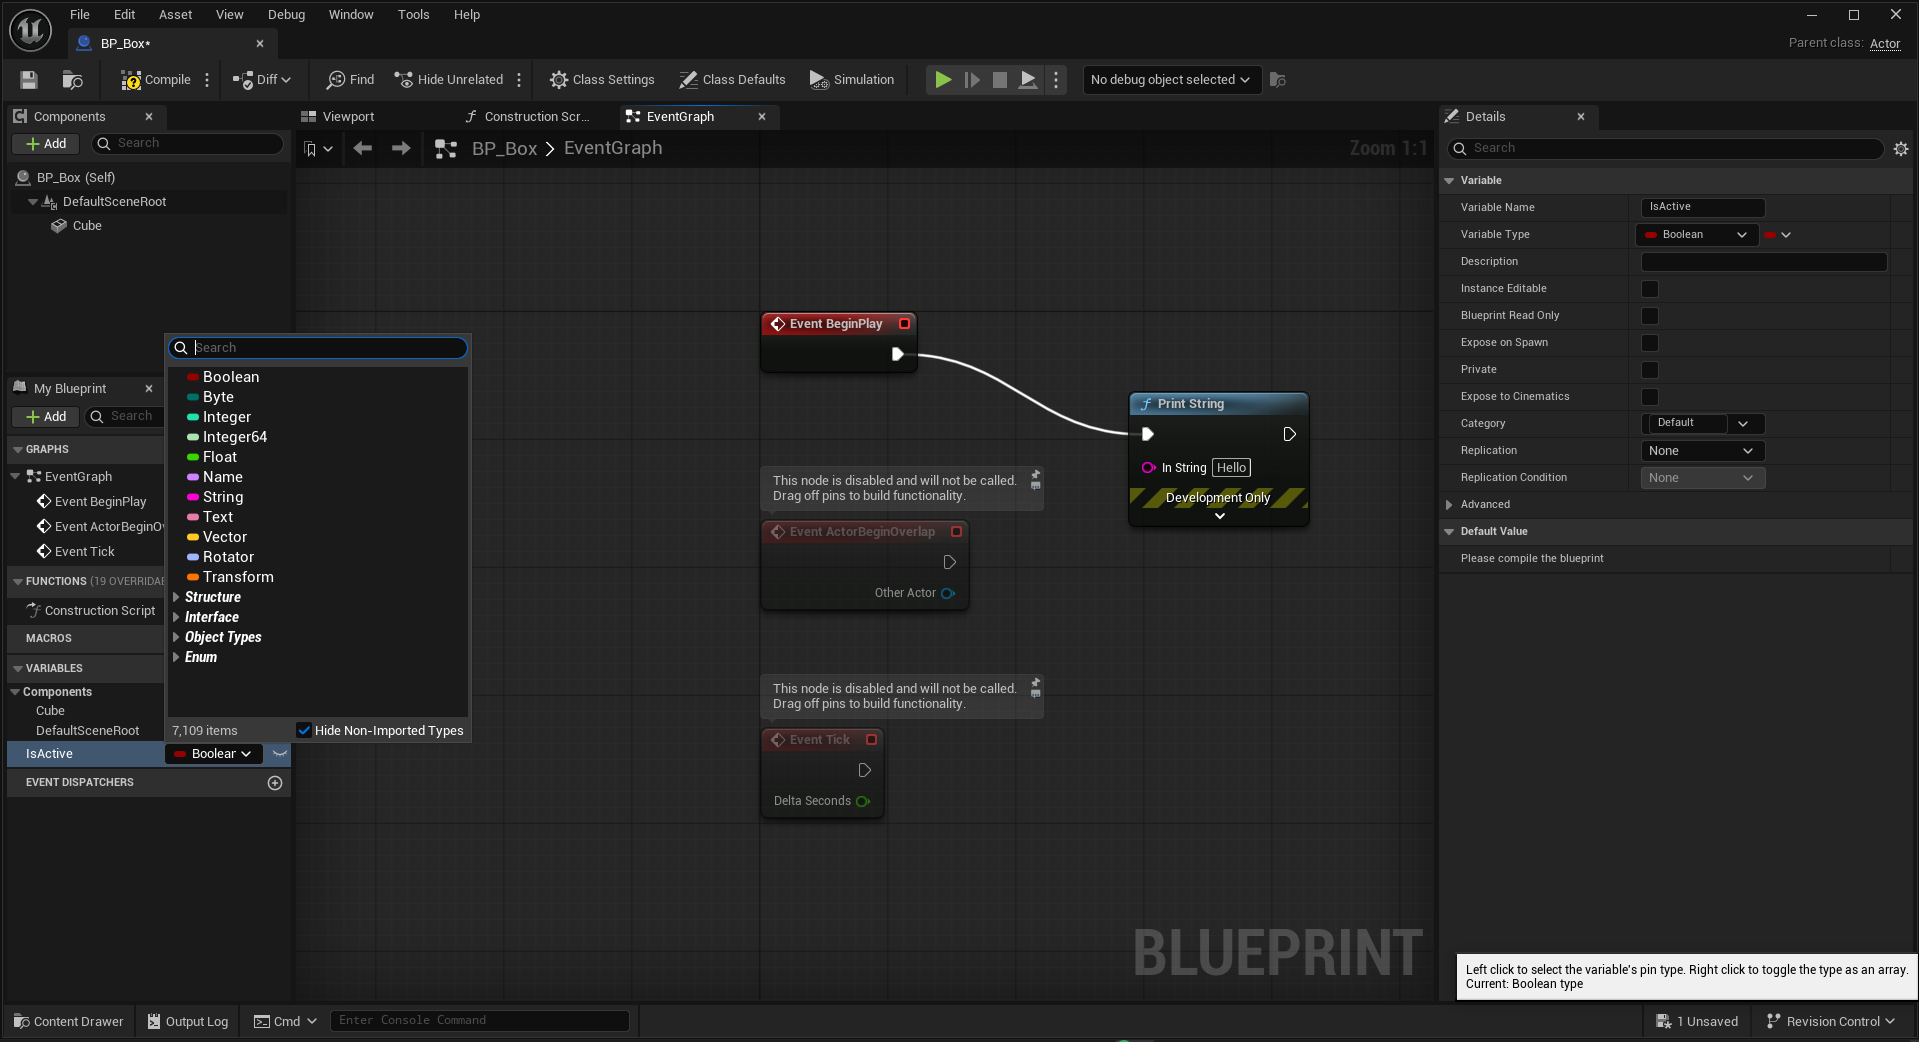
\includegraphics[width=0.9\textwidth]{images/ss-07-variabel-boolean.png}}
    \caption{Panel My Blueprint: variabel Boolean IsActive di BP\_Box beserta daftar tipe data yang tersedia.}
    \label{fig:ss-variable}
\end{figure}
\end{enumerate}

\subsection{Branch dan Input Keyboard}

\begin{enumerate}
    \item \textbf{Menambahkan node lewat klik kanan.} Area kosong Event Graph saya klik kanan lalu mengetik kata kunci seperti ``branch'', ``get'', ``set'', dan ``print string'' untuk memunculkan node yang dibutuhkan. Navigasi kanvas dilakukan dengan menahan klik kanan sambil menggerakkan mouse.

\begin{figure}[H]
    \centering
    \customfbox{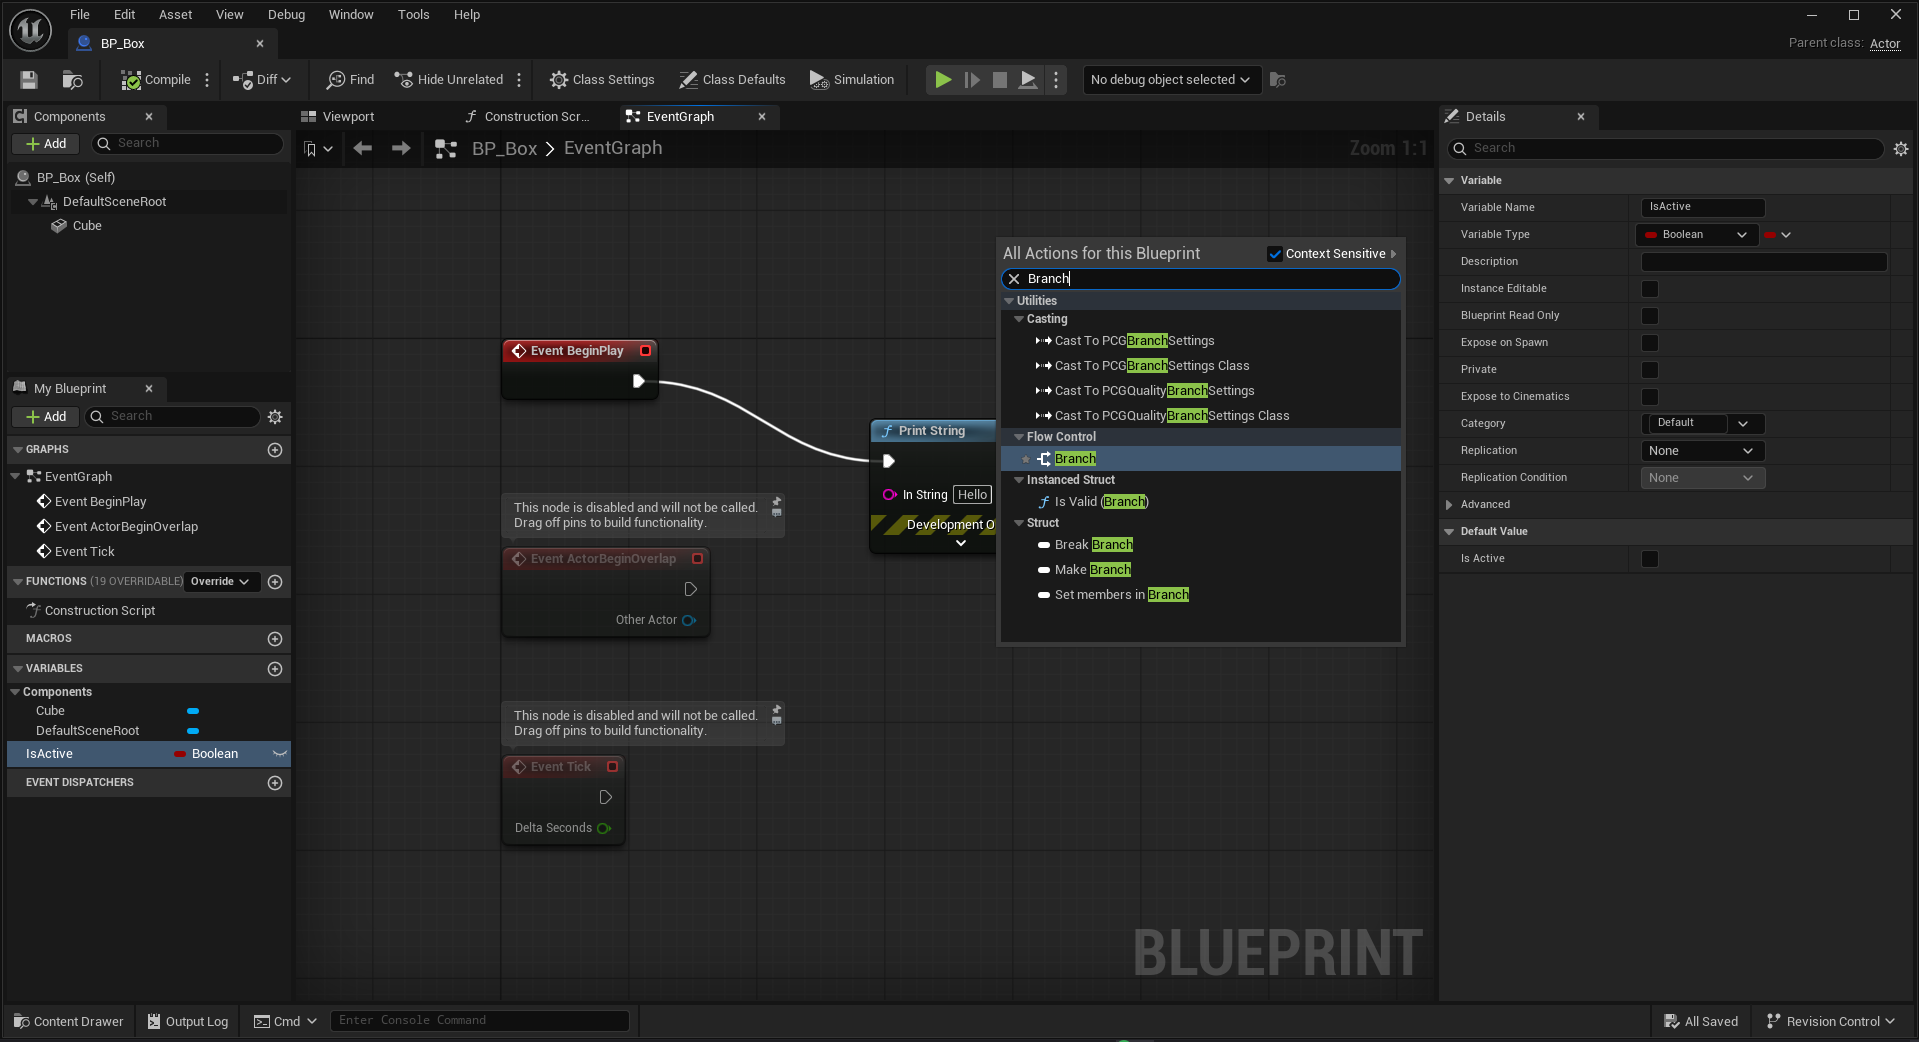
\includegraphics[width=0.9\textwidth]{images/ss-08-add-node-branch.png}}
    \caption{Menu klik kanan tambah node di Event Graph dengan kata kunci pencarian Branch.}
    \label{fig:ss-addnode}
\end{figure}

    \item \textbf{Merangkai Branch dengan Keyboard R.} Node \textbf{Event Tick} dihubungkan langsung ke node \textbf{Branch}. Input pemain ditangkap memakai node \textbf{Keyboard R} (kategori Input Events). Pin Pressed dan Released dipakai mengubah nilai variabel Boolean \textbf{IsActive} lewat node \textbf{SET} (True saat ditekan, False saat dilepas). Nilai tersebut kemudian dibaca dengan node \textbf{GET} dan diteruskan ke pin kondisi \textbf{Branch}. Dari pin True dan False, dua node \textbf{Print String} dipasang sehingga teks debug di layar berganti dinamis mengikuti status penekanan tombol R.

\begin{figure}[H]
    \centering
    \customfbox{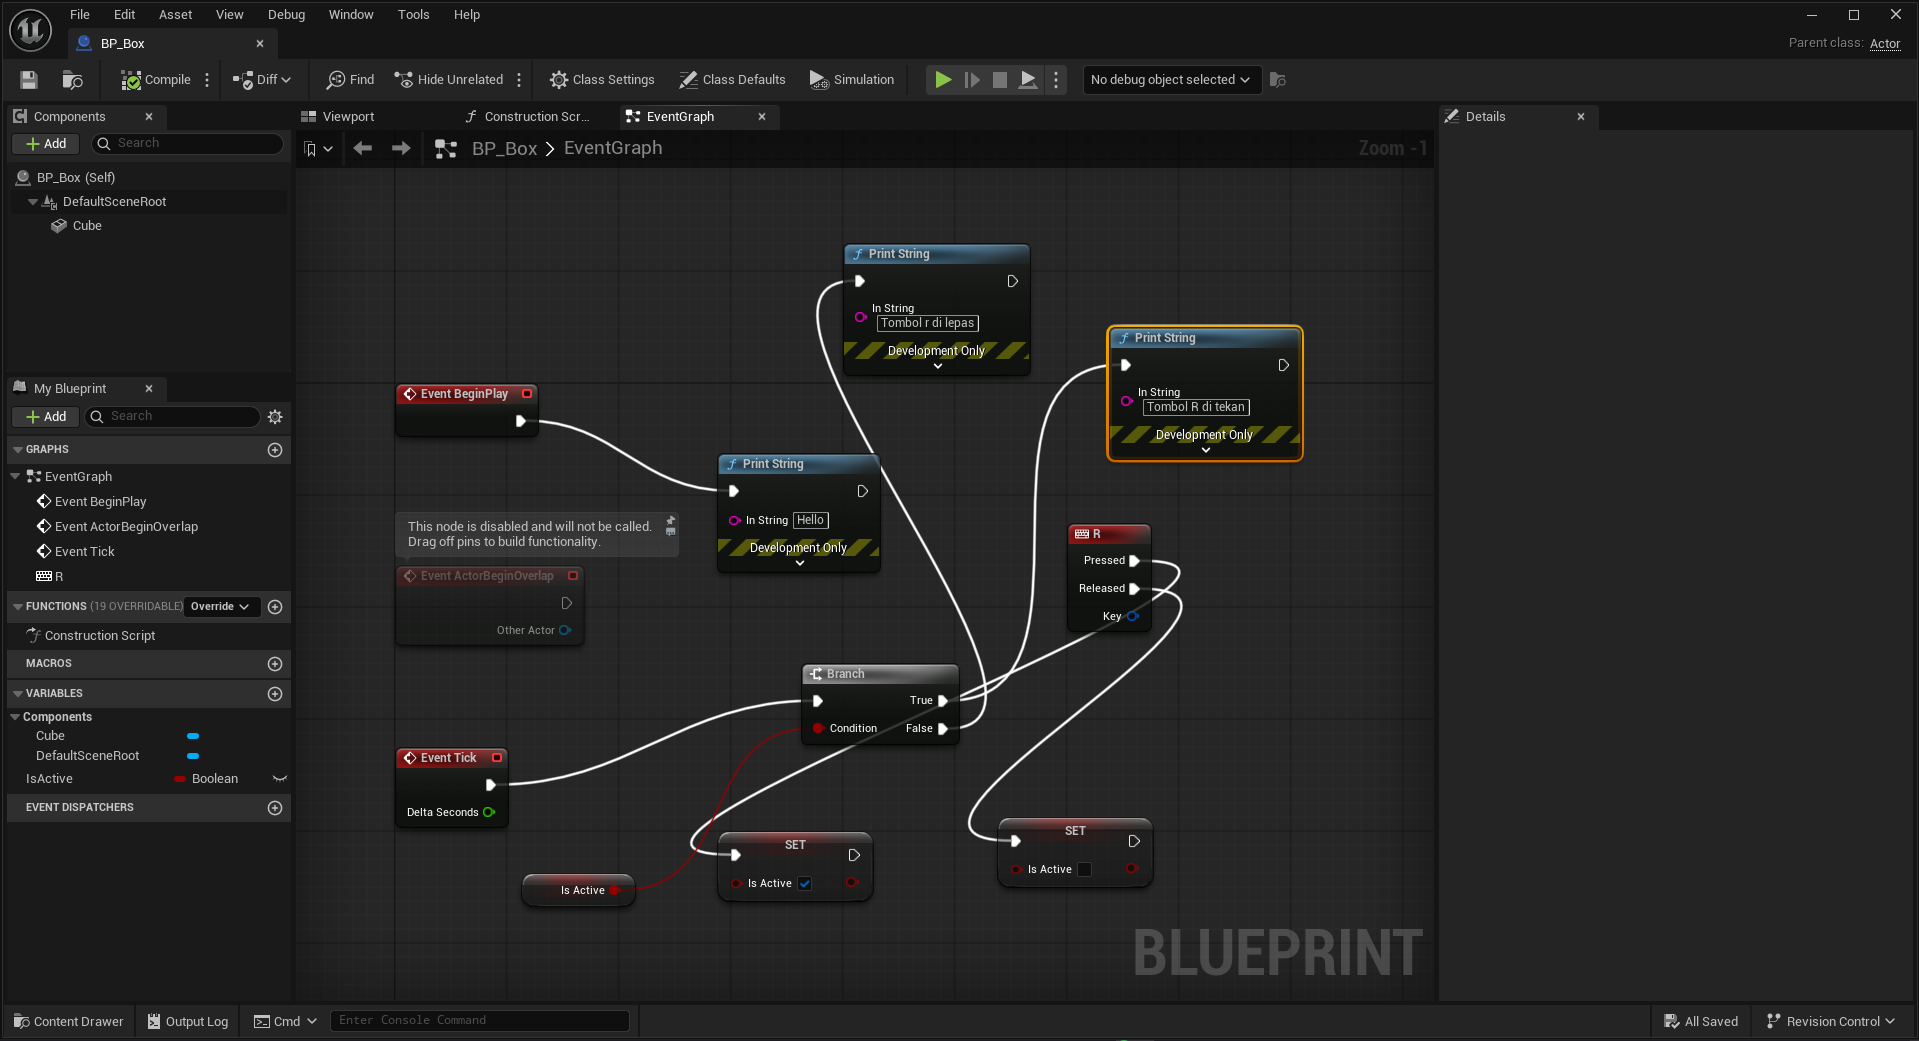
\includegraphics[width=0.9\textwidth]{images/ss-09-rangkaian-keyboard-branch.png}}
    \caption{Untaian logika Event Tick, Keyboard R, SET/GET IsActive, Branch, dan dua Print String.}
    \label{fig:ss-keyboard}
\end{figure}
\end{enumerate}

\subsection{Tugas: Aplikasi If/Else Pengubah Scale Real-Time}

\begin{enumerate}
    \item \textbf{Menambahkan variabel float ScaleTarget 0.1.} Sesuai instruksi tugas, variabel float bernama \textbf{ScaleTarget} saya tambahkan pada \texttt{BP\_Box} dengan default value \textbf{0.1} sebagai angka tujuan perubahan skala mesh.

\begin{figure}[H]
    \centering
    \customfbox{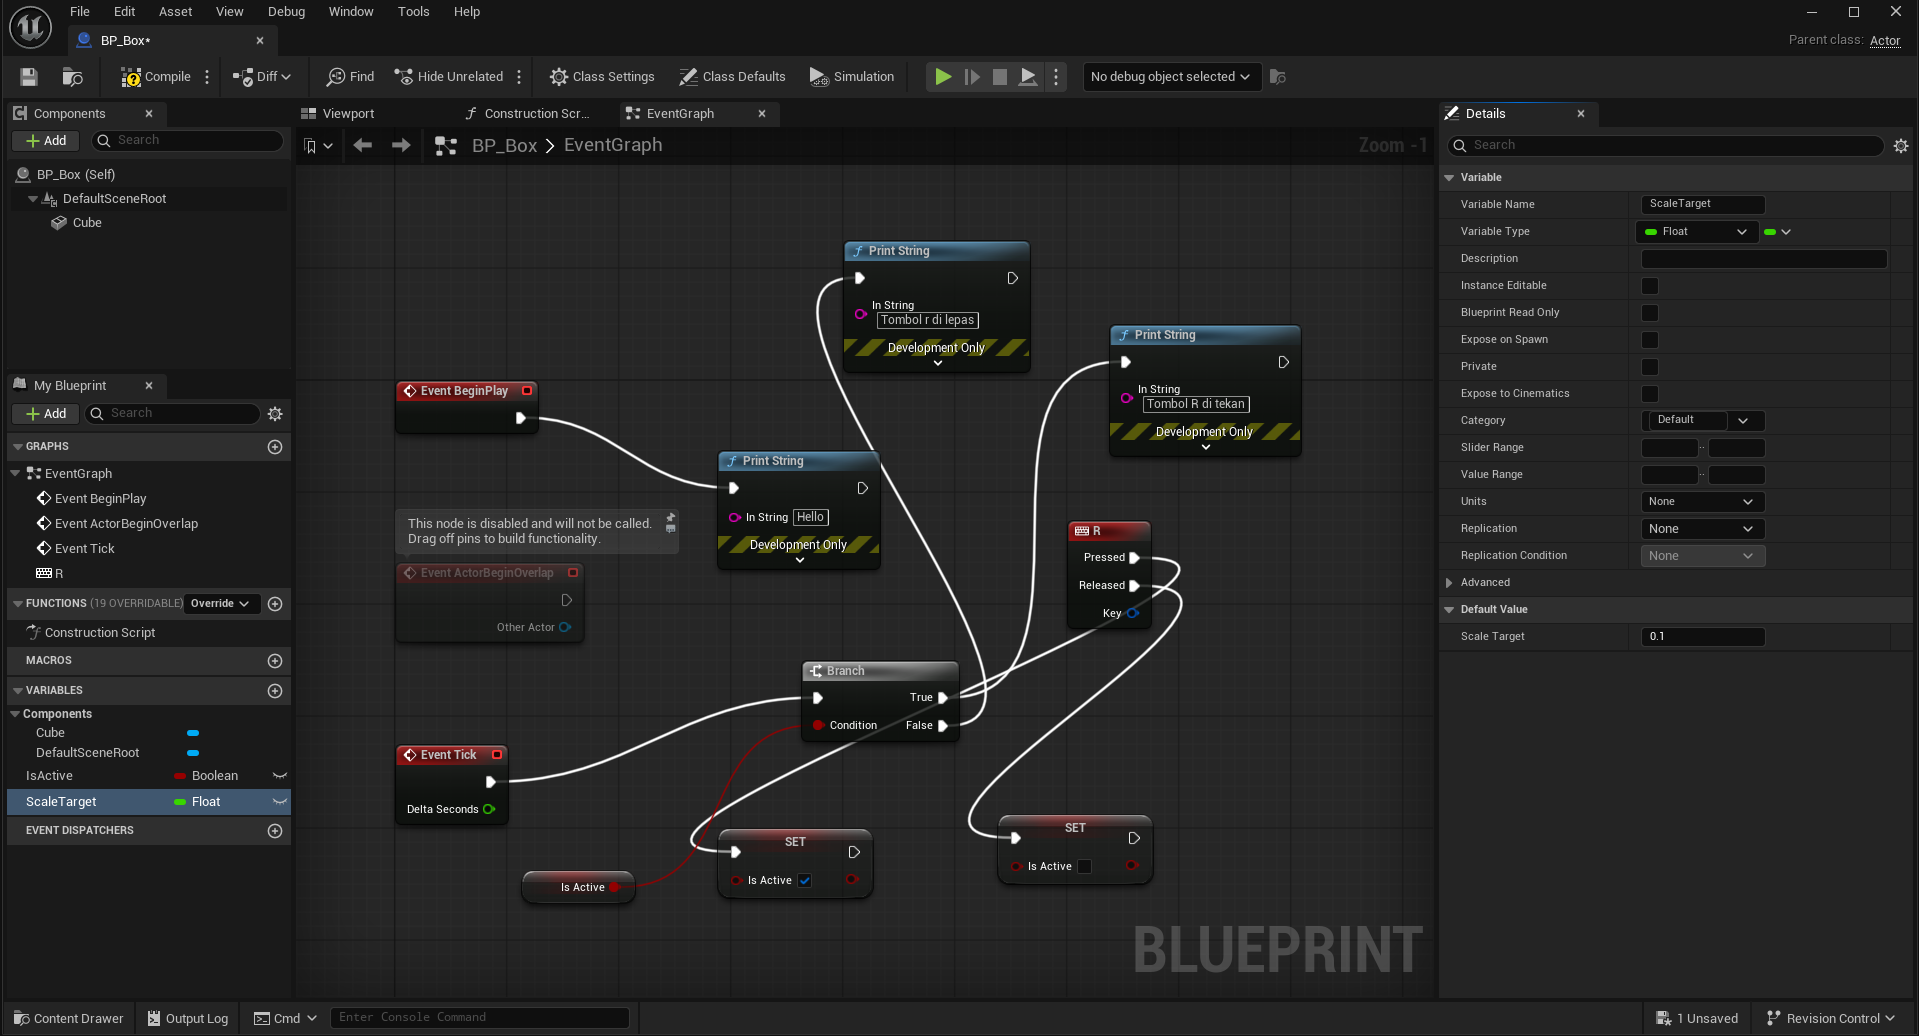
\includegraphics[width=0.9\textwidth]{images/ss-10-scale-target.png}}
    \caption{Variabel float ScaleTarget dengan default value 0.1 di panel My Blueprint milik BP\_Box.}
    \label{fig:ss-scaletarget}
\end{figure}

    \item \textbf{Merangkai Event Tick pengubah scale.} Kode pada Event Tick \texttt{BP\_Box} dihubungkan ke kalkulasi pengurangan nilai Scale mesh dengan \textit{ScaleTarget}. Nilai skala mesh dibaca dari komponen \textbf{Cube} lewat node \textbf{Get Relative Scale 3D}, dikurangi \textbf{ScaleTarget} melalui node operasi pengurangan yang pin bawahnya dikonversi ke float, lalu hasilnya diset kembali ke mesh lewat node \textbf{Set Relative Scale 3D}. Rangkaian ini dipicu saat tombol R ditekan sehingga perubahan skala terjadi secara real-time.

\begin{figure}[H]
    \centering
    \customfbox{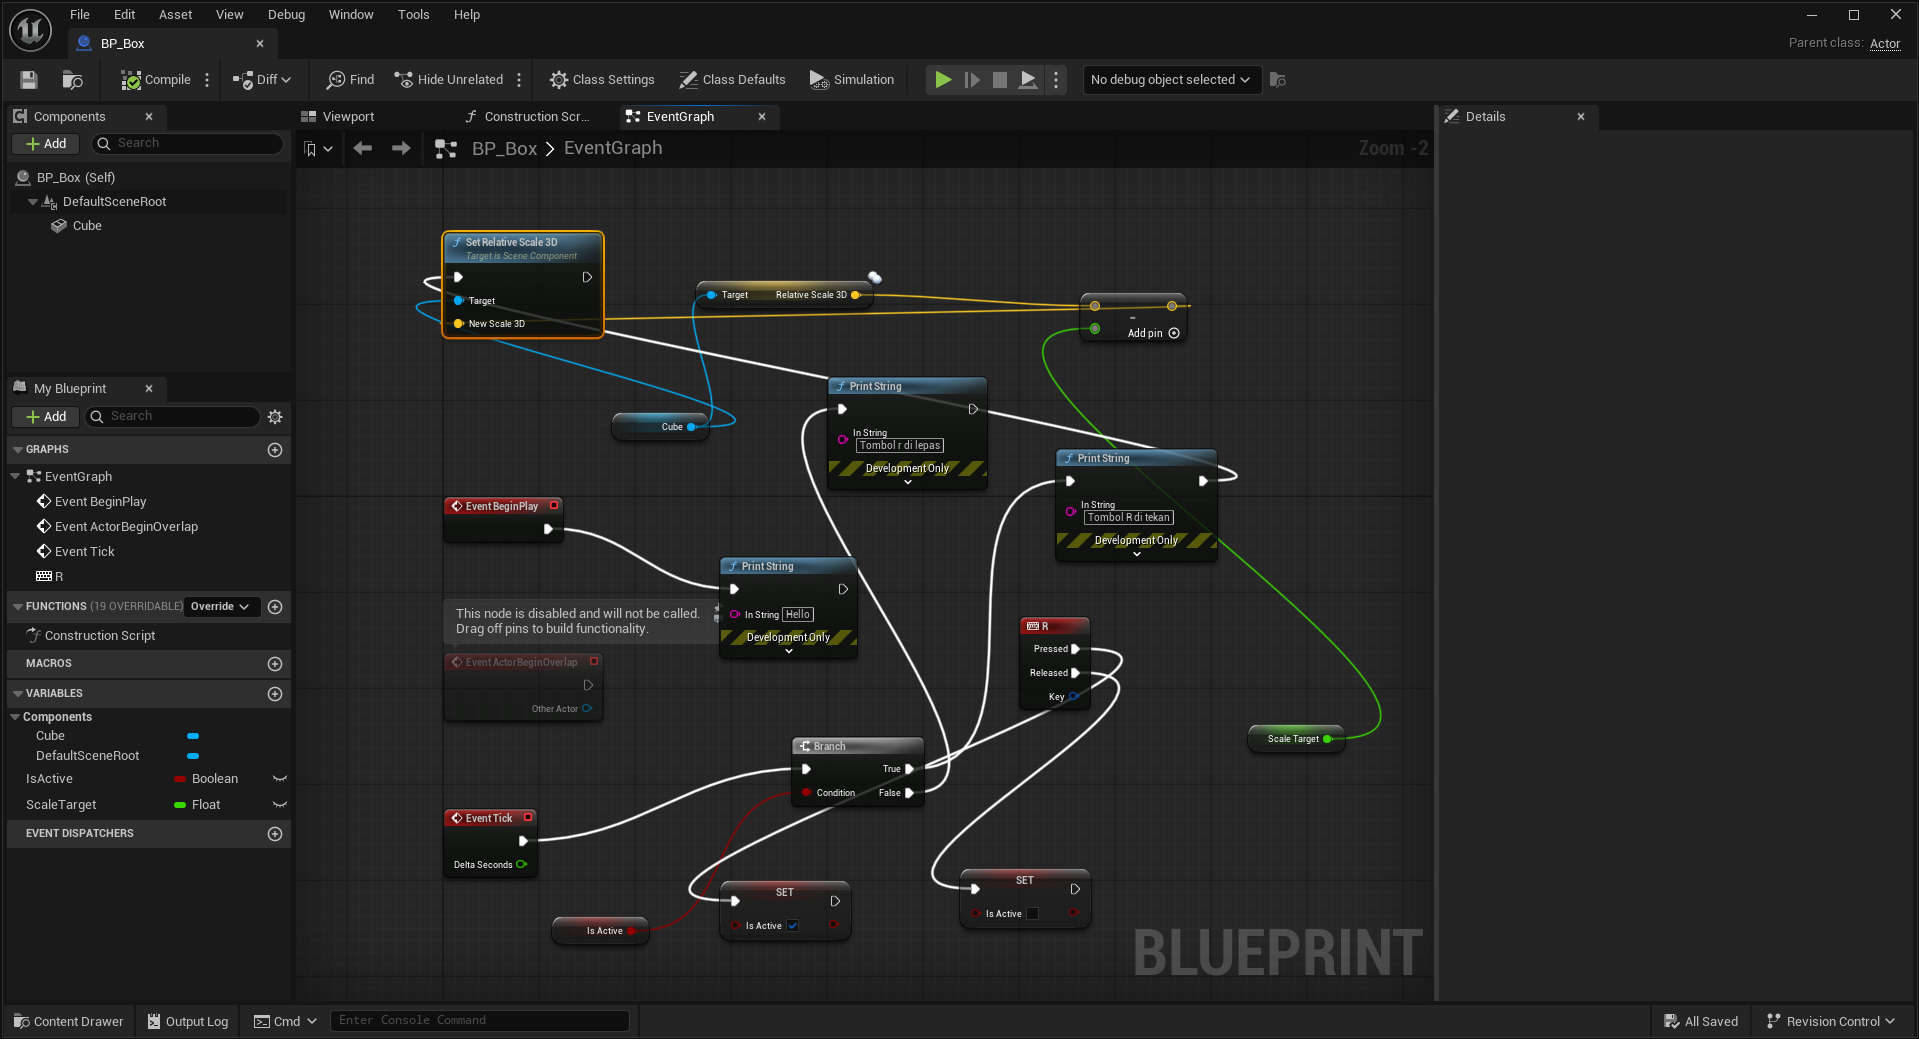
\includegraphics[width=0.9\textwidth]{images/ss-11-tugas-tick-scale.png}}
    \caption{Rangkaian Event Tick tugas: Scale mesh digeser real-time menuju 0.1 dengan Set Relative Scale 3D.}
    \label{fig:ss-tickscale}
\end{figure}
\end{enumerate}

\section{Hasil Akhir}
Di akhir praktikum, project \texttt{HAFIDZ\_535493\_PPG} sudah siap dari template Third Person lengkap dengan folder Maps, Level baru L\_Main, pencahayaan Env.\ Light Mixer, Landscape 7x7, dan Player Start. Blueprint \texttt{BP\_Box} berisi komponen Cube, variabel Boolean \texttt{IsActive}, dan variabel float \texttt{ScaleTarget} bernilai 0.1. Logika Branch dengan input Keyboard R mencetak teks debug secara real-time mengikuti status tombol (dilepas atau ditekan), dan rangkaian tugas mengubah Scale mesh secara langsung saat game di-Play.

\begin{figure}[H]
    \centering
    \customfbox{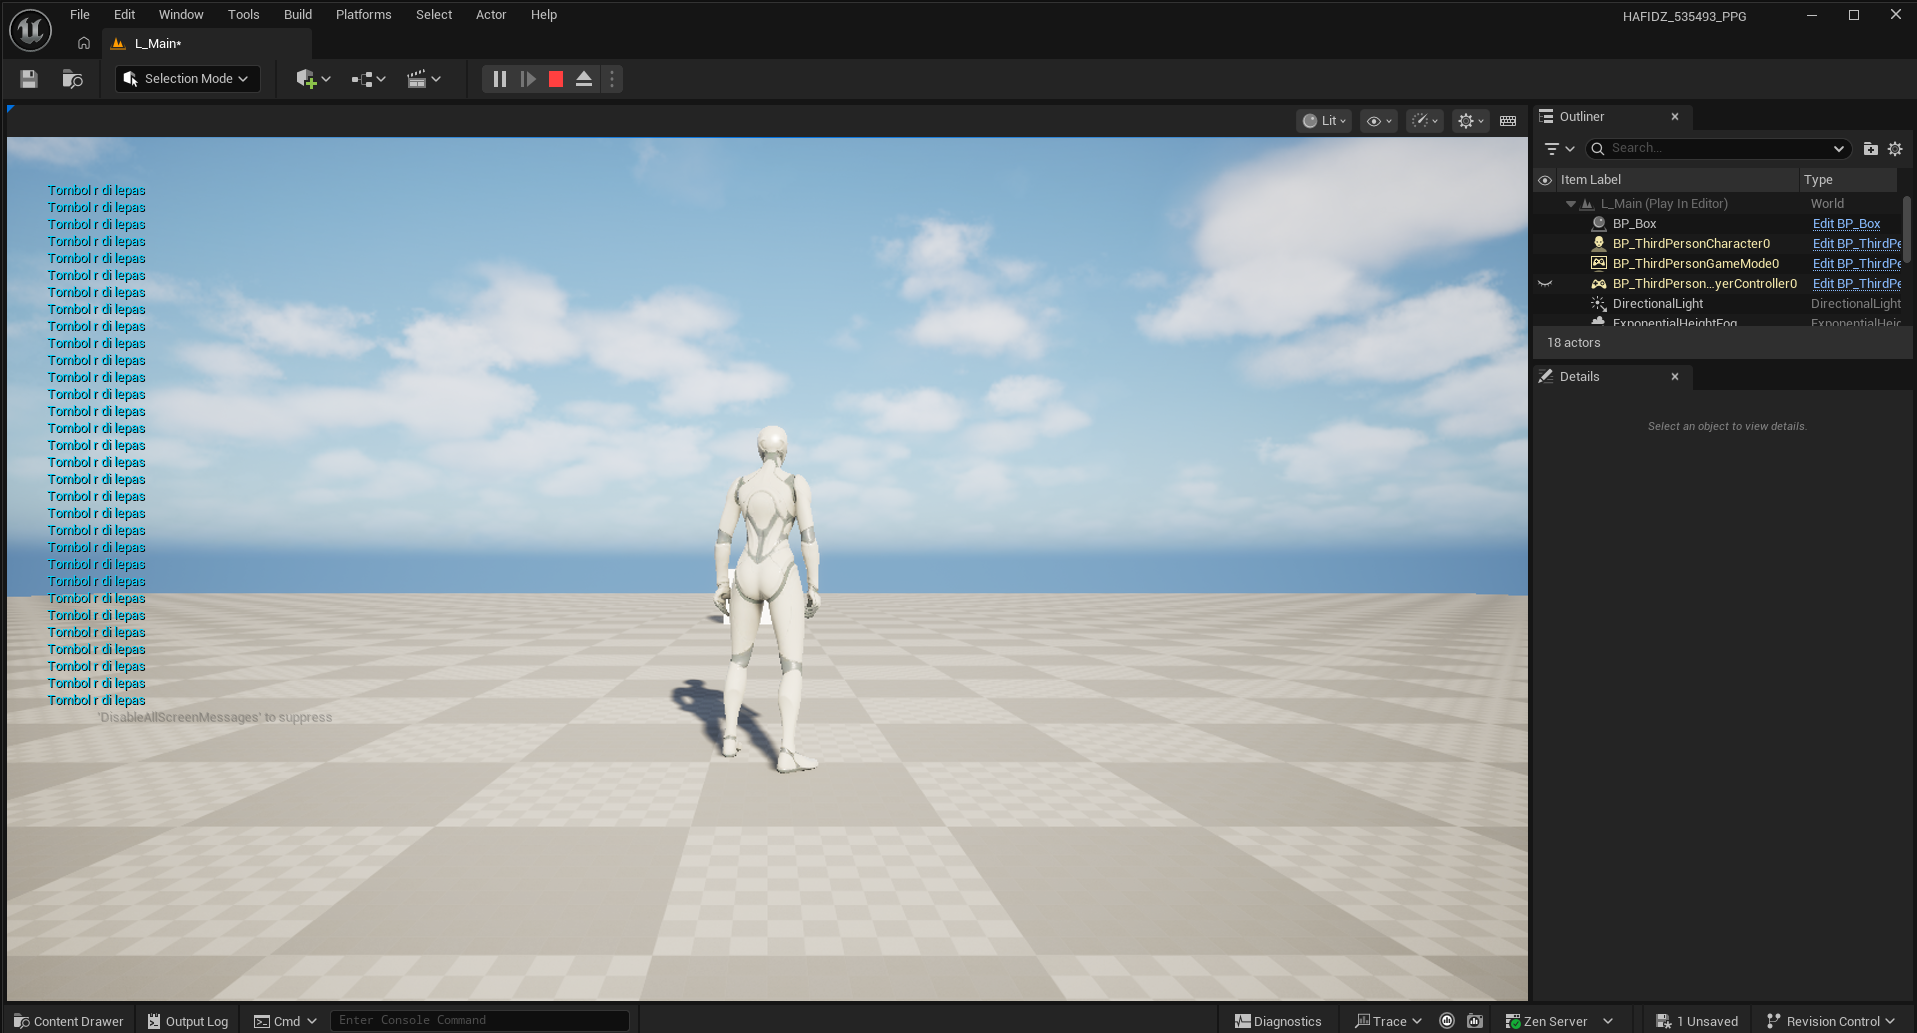
\includegraphics[width=0.9\textwidth]{images/ss-12-hasil-akhir-play.png}}
    \caption{Hasil akhir saat Play: BP\_Box di dunia, karakter spawn, dan teks debug Print String di layar.}
    \label{fig:hasil-akhir}
\end{figure}

Rangkaian ini menunjukkan instruksi modul dari pembuatan project sampai aplikasi if/else real-time sudah saya ikuti, sesuai ketentuan Format Tugas Modul 3 \cite{modul3}. Terakhir, semuanya disimpan dengan \texttt{CTRL+S}.

\clearpage

\chapter{Kesimpulan}
Template Third Person menjadi titik awal yang tepat untuk materi logika karena bersih dari kendala rigging karakter IntroToUnreal. Level kerja disiapkan dari awal mencakup folder Maps, level baru L\_Main, pencahayaan Env.\ Light Mixer, Landscape 7x7, dan Player Start sebagai titik spawn.

Alur kerja Blueprint juga dipahami secara terstruktur: file berawalan \texttt{BP\_} dengan komponen visual Cube, event BeginPlay yang berjalan satu kali dan Event Tick yang berjalan tiap frame, serta variabel Boolean yang didefinisikan dari panel My Blueprint. Node Branch terbukti berfungsi sebagai percabangan logika dengan dua keluaran True/False, dan input Keyboard R lengkap dengan Set/Get membuat teks debug berganti sesuai interaksi pemain.

Pada bagian tugas, variabel float \texttt{ScaleTarget} 0.1 dan konversi pin konektor ke float membuat Scale mesh bergeser secara real-time melalui node Set Relative Scale 3D. Pendekatan ini dicatat sebagai materi pembelajaran konsep logika if/else di Blueprint, sementara node kontrol alur lanjutan seperti Switch, Do Once, Flip Flop, dan Gate dipelajari mandiri sebagai bekal pembuatan mekanik game berikutnya.

\clearpage
\addcontentsline{toc}{chapter}{Daftar Pustaka}
\renewcommand{\bibname}{Daftar Pustaka}
\begin{thebibliography}{99}
    \bibitem{modul3} Modul Praktikum Pengembangan Game Pertemuan 3: Variable \& Condition, T.A. 2026/2027. Semester Gasal, Universitas Gadjah Mada.
    \bibitem{epic-unreal} Epic Games, ``Unreal Engine 5 Documentation'', 2026. [Online]. Tersedia: \url{https://dev.epicgames.com/documentation/unreal-engine/}.
    \bibitem{epic-levels} Epic Games, ``Levels in Unreal Engine'', 2026. [Online]. Tersedia: \url{https://dev.epicgames.com/documentation/en-us/unreal-engine/levels-in-unreal-engine}.
    \bibitem{epic-flow} Epic Games, ``Flow Control in Unreal Engine'', 2026. [Online]. Tersedia: \url{https://dev.epicgames.com/documentation/en-us/unreal-engine/flow-control-in-unreal-engine}.
    \bibitem{epic-input} Epic Games, ``Input in Unreal Engine'', 2026. [Online]. Tersedia: \url{https://dev.epicgames.com/documentation/en-us/unreal-engine/input-in-unreal-engine}.
    \bibitem{epic-actors} Epic Games, ``Actors in Unreal Engine'', 2026. [Online]. Tersedia: \url{https://dev.epicgames.com/documentation/en-us/unreal-engine/actors-in-unreal-engine}.
    \bibitem{epic-place} Epic Games, ``Place Actors and Geometry in Unreal Engine'', 2026. [Online]. Tersedia: \url{https://dev.epicgames.com/documentation/en-us/unreal-engine/place-actors-and-geometry-in-unreal-engine}.
    \bibitem{epic-running} Epic Games, ``Running Unreal Engine'', 2026. [Online]. Tersedia: \url{https://dev.epicgames.com/documentation/en-us/unreal-engine/running-unreal-engine}.
    \bibitem{epic-naming} Epic Games, ``Recommended Asset Naming Conventions in Unreal Engine Projects'', 2026. [Online]. Tersedia: \url{https://dev.epicgames.com/documentation/en-us/unreal-engine/recommended-asset-naming-conventions-in-unreal-engine-projects}.
    \bibitem{epic-variables} Epic Games, ``Blueprint Variables in Unreal Engine'', 2026. [Online]. Tersedia: \url{https://dev.epicgames.com/documentation/en-us/unreal-engine/blueprint-variables-in-unreal-engine}.
\end{thebibliography}

\end{document}
